\section{利器善事}
古人云:“工欲善其事,必先利其器”,一套良好的配置往往事半功倍。\TeX 的编译器,单线程工作,对单核性能要求较高,在选购电脑时CPU主频不宜过低。硬盘的读写很大程度上影响文档编译的时间,推荐上nvme固态硬盘,另外在相同的配置下,Linux下的I/O性能更好,推荐使用Linux系统,本套解决方案都是在Linux下完成,使用windows的用户请自行参考修改。

选择一个多功能的鼠标极大有益于提高工作效率,我使用的是罗技G502,主要优点如下:
\begin{itemize}
	\item 
	共有11个按键,方便配置各种不同的功能。
	\item 
	板载内存,一次修改,多处使用,不同配置,随时切换。
	\item 
	滚轮有极速模式,方便快速浏览。
\end{itemize}
注意,罗技的鼠标官方没有提供Linux下的配置软件,有两种解决方法,一是在windows下修改好后再在Linux下使用;二是在Linux下使用piper软件来设置。关于piper软件的安装和使用请参看piper官方文档的说明。图 \ref{fig:screenshot001} 是piper软件的使用截图。
% TODO: \usepackage{graphicx} required
\begin{figure}[h!]
	\centering
	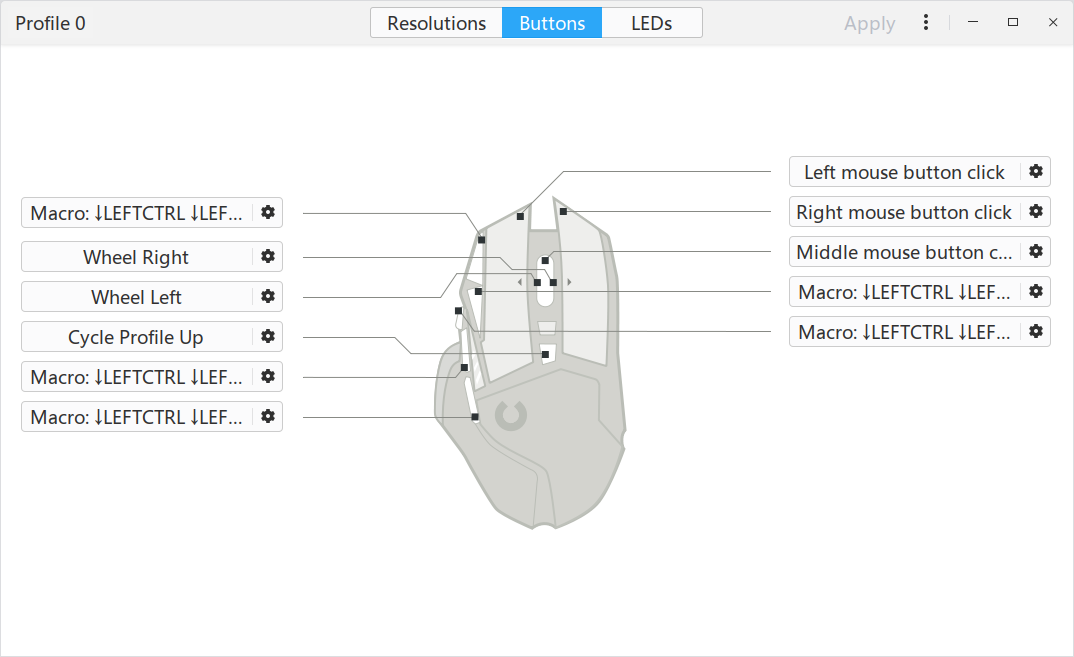
\includegraphics[width=0.7\linewidth]{picture/screenshot001}
	\caption{罗技鼠标的设置}
	\label{fig:screenshot001}
\end{figure}

在各种文档的转化里属扫描版的PDF文档最难,网上提供的扫描版质量参差不齐,最好购置一台专业的扫描仪,获得原始的高清文档,一般要求是分辨率600dpi,彩色扫描。另外,由于 \TeX 文档需要不时编译查看效果,显示器需要足够宽大;还有后面由于需要截图,而截图的分辨率基本取决于你显示器的分辨率,故能上2k或4k的显示器更好。\footnote{当你的显示器分辨率不够,又需要获得高分辨率的截图时,若显卡可以的话,可使用xrand修改输出分辨率,再对输出的图像采用缩放操作即可。}

